\documentclass{NEWSTYLE}

\begin{document}
	
	Hello World!
	
	%All humans need water and I would like
	%to include this concept in my arguments.
	We all need \ce{H2O}.
	
	%Uranium 235 is toxic, which is why I don’t want to consume it...
	I’m less fussed about \ce{^{235}_{92}U+}.

\chapter{2222222}
\section{bbb}

\begin{itemize}
	\item cat
	\item dog
	\item horse
\end{itemize}

\begin{enumerate}
	\item cat
	\item dog
	\item horse
\end{enumerate}

\begin{description}
	\item[Cat] a lovely furry creature with a cute nose and whiskers.
	\item[Dog] Another furry creature that smells rather well;
	its olfactory power stems from its nasal dampness.
	\item [Horse] A large stinky creature with sideways facing eyes.
\end{description}

\begin{center}
	
\begin{math}
\imath\hbar\frac{\partial}{\partial t}\Phi\left( x,t \right) =
\hat{H}\Phi \left( x,t \right)
\end{math}


\begin{equation}
y(\left(t\right)= \sin \left(\frac{{\alpha}t}{2\pi} + \phi_0\right)
\end{equation}

\begin{eqnarray}
A\left( x\right) & = & \frac{x^2+2x+1}{1+x} \\
& = & \frac{\left(x+1\right)\left(x+1\right)}{1+x} \nonumber\\
& = & x+1 \nonumber\\
B(x,t) & = & \frac{e^{\left(\imath\omega_0 t + kx\right)}}{4\pi\epsilon_0}
\end{eqnarray}

\ce{CO2 + C -> 2CO}

\ce{CO2 + C <- 2CO}

\ce{CO2 + C <=> 2CO}

\ce{A-B=C#D\sbond E\dbond F\tbond G}

\ce{$x\,$ Na(NH4)HPO4 ->[\Delta] (NaPO3)_{$x$} + $x\,$ NH3 ^ + $x\,$ H2O}

\begin{equation}
\ce{CO2 + C <=> 2CO}
\end{equation}

\chapter{cvcvcvc}

\begin{tabular}{lcr}
	anchovy & banana & carrot \\
	dog & apple & fennel \\
	goat & strawberry & potato
\end{tabular}

\begin{tabular}{cccc}
	anchovy & banana & carrot & Johnny\\
	dog & apple & fennel & Pete\\
	goat & strawberry & potato &
\end{tabular}

\begin{tabular}{|c|c|c|c|}
	anchovy & banana & carrot & Johnny\\
	dog & apple & fennel & Pete\\
	goat & strawberry & potato &
\end{tabular}

\begin{tabular}{cccc}
	\toprule
	Ingredient 1 & Ingredient 2 & Ingredient 3 & Source \\
	\cmidrule(){1-4}
	anchovy & banana & carrot & Johnny\\
	dog & apple & fennel & Pete\\
	goat & strawberry & potato & \\
	\bottomrule
\end{tabular}

\begin{tabular}{ccccc}
	\toprule
	Recipe Version & Ingredient 1 & Ingredient 2 & Ingredient 3 & Source \\
	\cmidrule(lr){1-1}
	\cmidrule(l){2-2}
	\cmidrule(){3-3}
	\cmidrule(r){4-4}
	\cmidrule(lr){5-5}
	10.1 & anchovy & banana & carrot & Johnny\\
	1.34 & dog & apple & fennel & Pete\\
	709.23 & goat & strawberry & potato & \\
	\bottomrule
\end{tabular}

\begin{tabular}{D{.}{\cdot}{4,4}cccc}
	\toprule
	Recipe Version & Ingredient 1 & Ingredient 2 & Ingredient 3 & Source \\
	\cmidrule(lr){1-2}
	\cmidrule(lr){3-3}
	\cmidrule(lr){4-4}
	\cmidrule(lr){5-5}
	10.1 & anchovy & banana & carrot & Johnny\\
	1.34 & dog & apple & fennel & Pete\\
	709.23 & goat & strawberry & potato & \\
	\bottomrule
\end{tabular}

\begin{tabular}{D{.}{\cdot}{4,4}cccc}
	\toprule
	\multicolumn{1}{c}{Recipe Version} & Ingredient 1 & Ingredient 2 & Ingredient 3 & Source \\
	\cmidrule(lr){1-1}
	\cmidrule(lr){2-2}
	\cmidrule(lr){3-3}
	\cmidrule(lr){4-4}
	\cmidrule(lr){5-5}
	10.1 & anchovy & banana & carrot & Johnny\\
	1.34 & dog & apple & fennel & Pete\\
	709.23 & goat & strawberry & potato & \\
	\bottomrule
\end{tabular}

\begin{table}[!h]
	\centering
	\begin{tabular}{D{.}{\cdot}{4,4}cccc}
		\toprule
		\multicolumn{1}{c}{Recipe Version}& Ingredient 1 & Ingredient 2 & Ingredient 3 & Source\\
		\cmidrule(lr){1-1}
		\cmidrule(lr){2-2}
		\cmidrule(lr){3-3}
		\cmidrule(lr){4-4}
		\cmidrule(lr){5-5}
		10.1 & anchovy & banana & carrot & Johnny\\
		1.34 & dog & apple & fennel & Pete\\
		709.23 & goat & strawberry & potato & \\
		\bottomrule
	\end{tabular}
	\caption[Table of Banned Recipes]{Recipes that ought to be banned.}
	\label{tab:Recipes}
\end{table}

\begin{figure}[!ht]
	\centering
	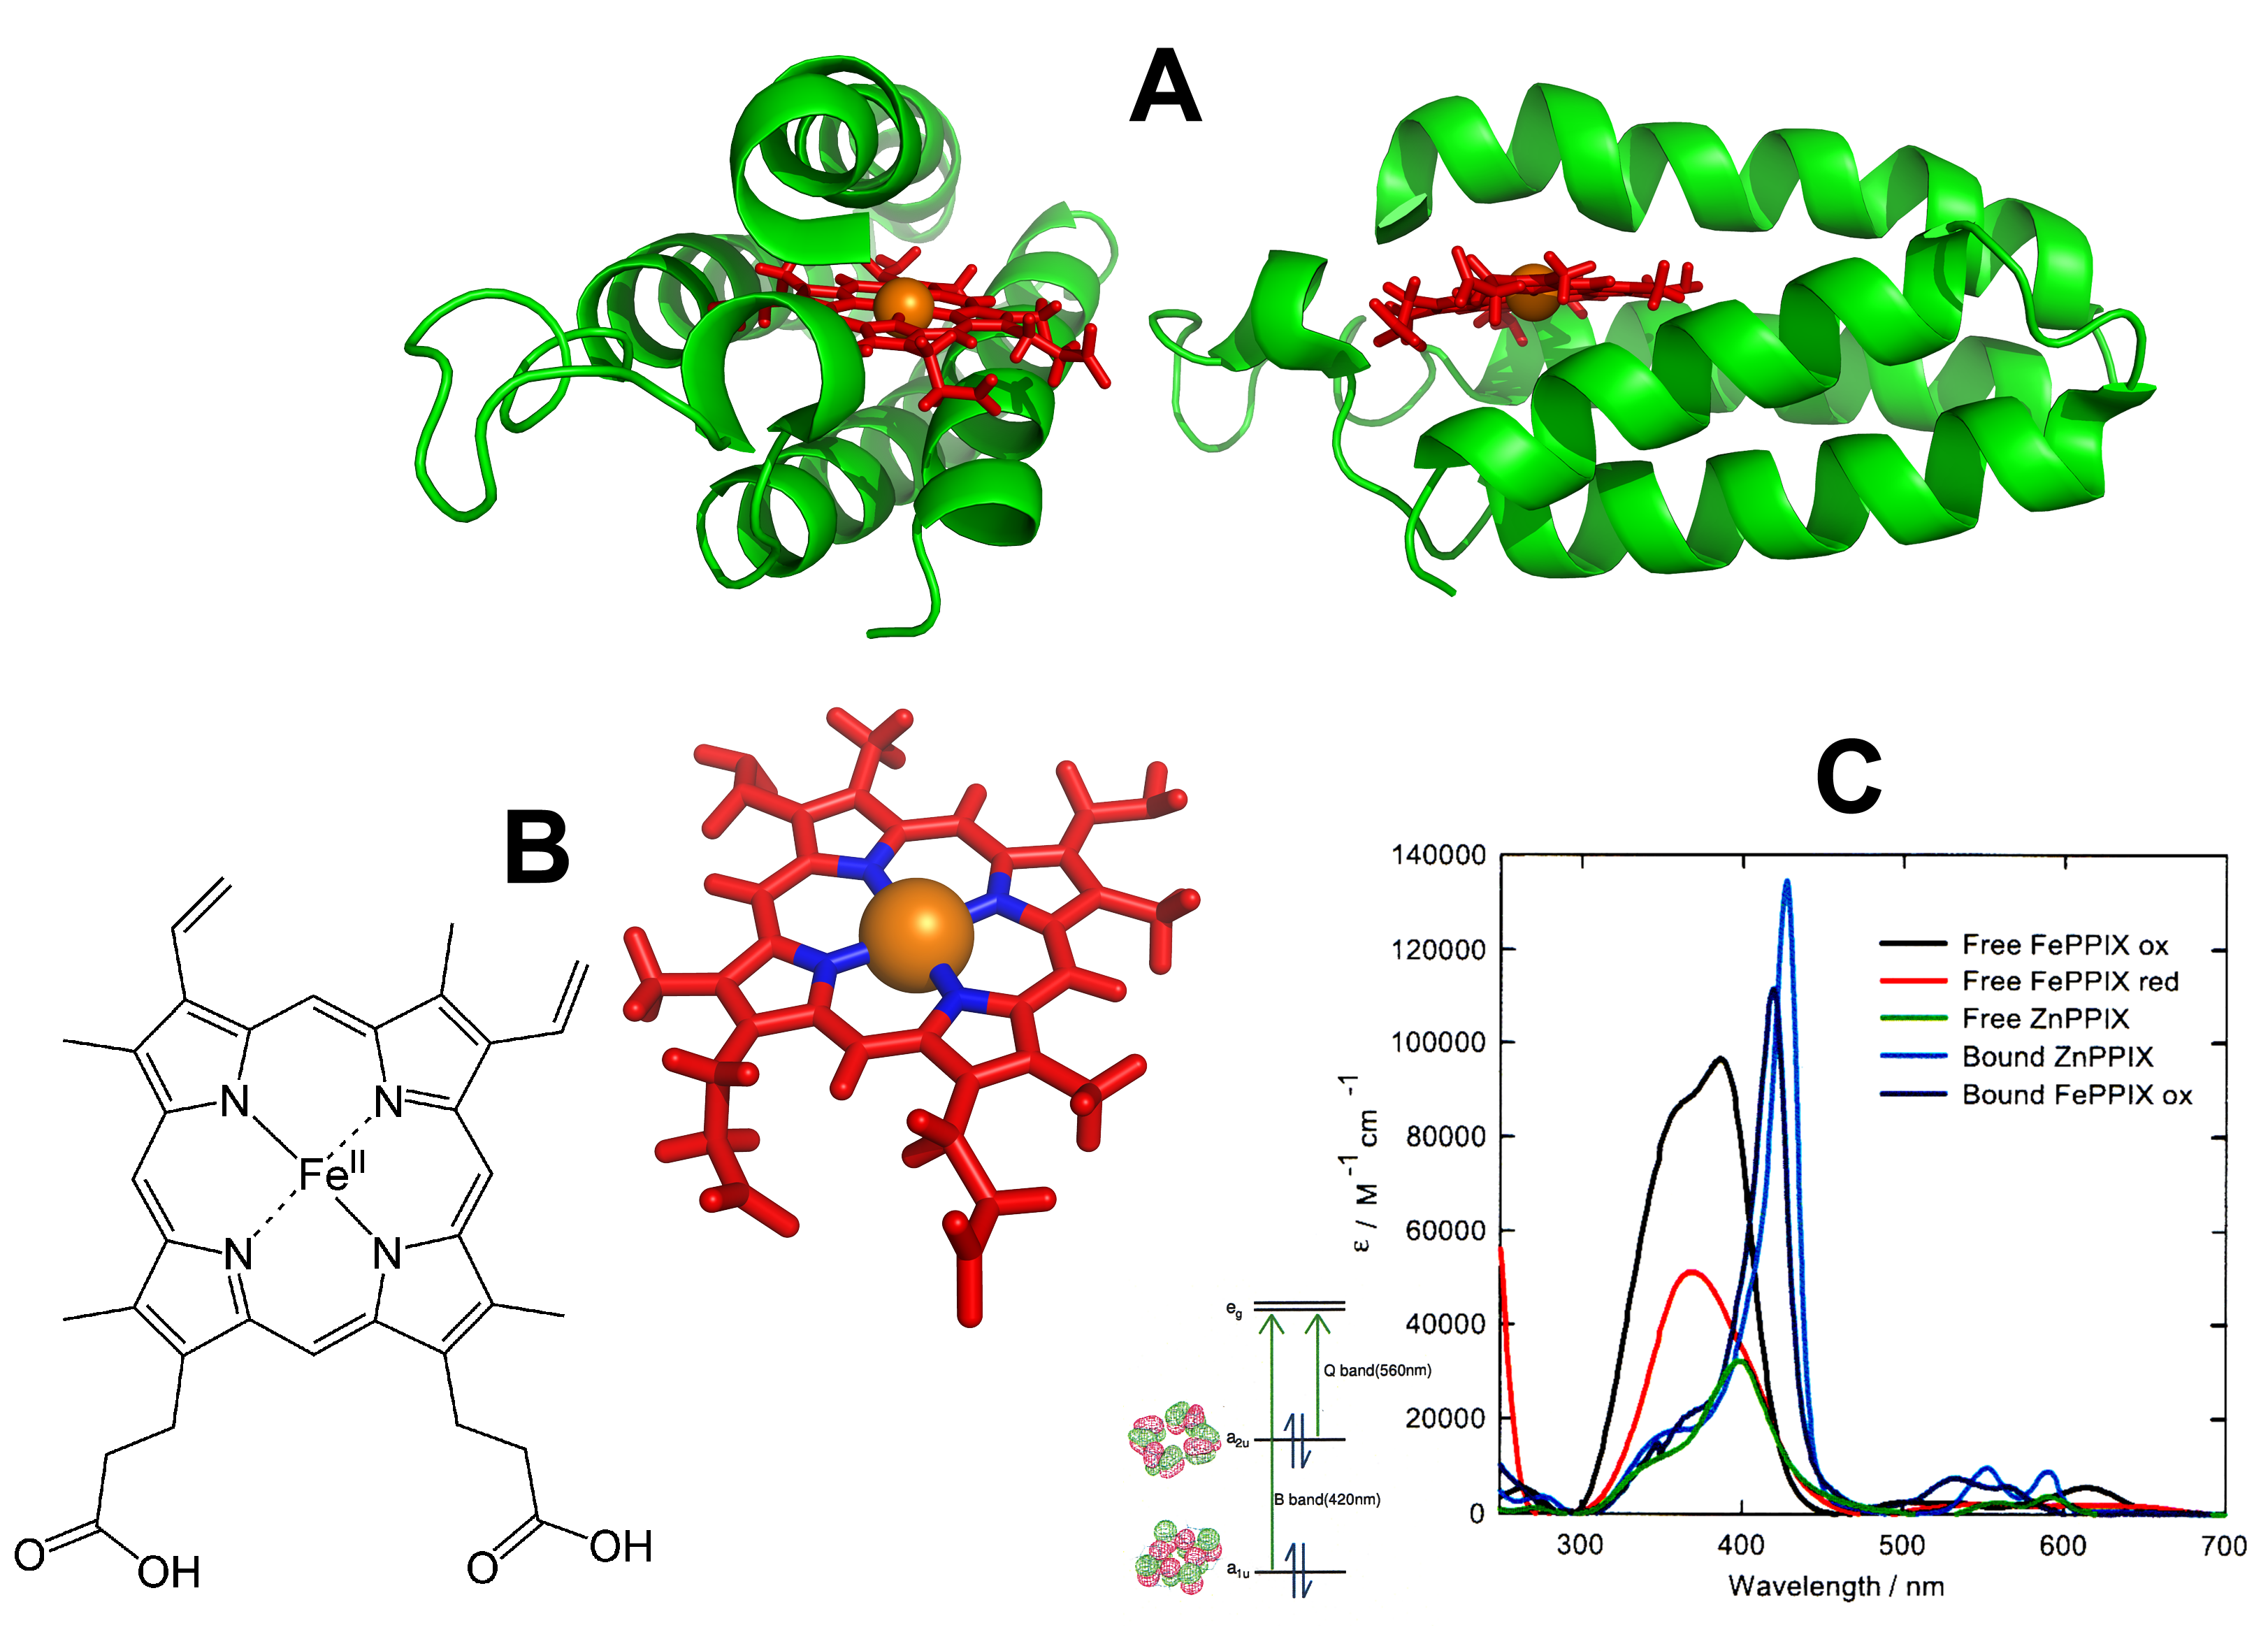
\includegraphics[width=1.0\textwidth]{Images/haemStructure.png}
	\caption[Haem Structure]{A fancy image.}
	\label{fig:haemStructure}
\end{figure}
\end{center}

REF

fig\ref{fig:haemStructure}

table\ref{tab:Recipes}

\bibliographystyle{Bibliography/cjfthesisv1}

hello\cite{Gazit2002,Channon2009,Horcas2007,Jones2003,Parsons2010,Stott2009}

\bibliography{Bibliography/LaTeXCourseBib}


\end{document}











